\section{Edge Execution and Compression}
\label{sec:edge}

\begin{figure}[!t]
\centering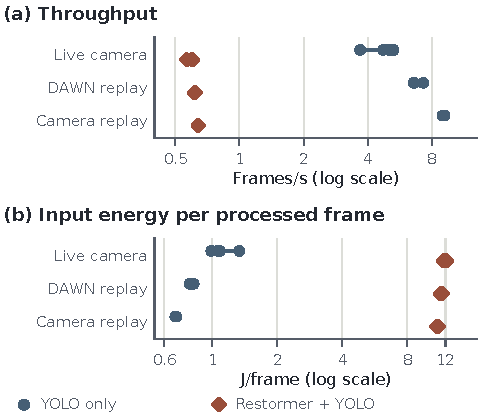
\includegraphics[width=\linewidth]{figures/nano_runtime.pdf}
\caption{Original Jetson Nano throughput and board input energy. Each point is one weather condition. The lines span conditions within a workload. Live application FPS and replay FPS have different timing boundaries. Energy uses integrated board input power divided by processed frames.}
\label{fig:nano-runtime}
\end{figure}

\paragraph{Measured Nano execution.}
Figure~\ref{fig:nano-runtime} separates live, labelled replay, and saved-camera replay. In DAWN replay, YOLO alone reaches 6.55--7.28 FPS with median pipeline latency of 129.2--147.2\,ms. Adding the $128\times128$ restorer yields 0.61--0.62 FPS and 1,596.7--1,619.6\,ms. Board input energy rises from 0.78--0.82 to 11.35--11.59\,J/frame, about 14--15 times more across weather subsets. The live cascade runs at 0.57--0.60 FPS. Live throughput includes capture, weather generation, display, and application overhead. Replay isolates the processing path. Power integrates the board input rail without subtracting idle power. Short, single-run windows constrain runtime and energy estimates (Supplementary Appendix~D).

\paragraph{Conversion and deployment.}
The measured cascade uses FP32 YOLOv8n and a mixed FP16/FP32 Restormer on the original 4\,GB Jetson Nano with TensorRT 8.2.1.8. Its detector and restorer pass three and four numerical fixtures, respectively. Lower-precision weights can reduce storage and memory traffic when the runtime packs and executes them. The separate 8-bit weight grid retains FP32 execution and storage at 105,748,439 bytes. Fog and smoke exceed its output RMSE limit at 0.00618 and 0.00464. The 8-bit candidate and pruning controls remain offline screens (Supplementary Appendix~C).
